\section{Экзамен}

\subsection{Базы данных и системы управления базами данных. Определения, основные функции и классификация}

\textbf{База данных} (БД) ---  самодокументированное собрание интегрированных записей.

\begin{enumerate}
	\item БД является самодокументированной, т.е. она содержит описание собственной структуры. Это описание называется словарем данных, каталогом данных или метаданными.
	\item БД является собранием интегрированных записей, т.е. она содержит:
	\begin{itemize}
		\item файлы данных;
		\item метаданные (данные о данных);
		\item индексы, которые представляют связи между данными, а также служат для повышения производительности приложений базы данных;
		\item метаданные приложения.
	\end{itemize}
	\item БД является информационной моделью пользовательской модели предметной области.
\end{enumerate}

\textbf{OLAP} --- online analtyc proccesing (операциооные данные) чтение, вставка, удаление, мин время отклика.

\textbf{OLTP} --- online transaction proccessing (перманентые данные) вставка, удаление, обнровление, гарантия изменения информации.

\begin{table}[ht!]
	\begin{center}
		\caption{}
		\label{tbl:best}
		\begin{tabular}{|c|c|}
			\hline
			OLAP & OLTP \\
			\hline
			чтение & вставка, удаление, обновление \\
			\hline
			минимальное время отклика & минимальное время вставки, удаление, обновление \\
			\hline
		\end{tabular}
	\end{center}
\end{table}

\textbf{Транзакции} --- либо все действия, либо никакие действия.


\textbf{Любая бд хранит}:

\begin{enumerate}
	\item метаданные (данные о данных);
	\item файлы данных,
	\item Индексы (indexes), которые представляют связи между данными,  a также служат для повышения производительности приложений базы данных.
	\item Может содержать метаданные приложений (application metadata).
\end{enumerate}

\textbf{Основные храктеристики, требования}

\begin{enumerate}
	\item \textbf{Неизбыточность данных} --- каждое данное присутствует в БД в единственном экземпляре.
	\item \textbf{Совместное использование данных} многими пользователями.
	\item \textbf{Эффективность доступа} к БД - высокое быстродействие, т. е. малое время отклика на запрос.
	\item \textbf{Целостность данных} --- соответствие имеющейся в БД информации её внутренней логике, структуре и всем явно заданным правилам.
	\item \textbf{Безопасность данных} --- защита данных от преднамеренного или непреднамеренного искажения или разрушения данных.
	\item \textbf{Восстановление данных} после программных и аппаратных сбоев.
	\item \textbf{Независимость данных} от прикладных программ.
\end{enumerate}

\textbf{Система баз данных} (СБД) --- совокупность одной или нескольких баз данных и комплекса информационных, программных и технических средств, обеспечивающих накопление, обновление, корректировку и многоаспектное использование данных в интересах пользователей.

\textit{Система управления базами данных} (СУБД) --- приложение, обеспечивающее создание, хранение, обновление и поиск информации в базах данных.

\subsubsection{Основные функции СУБД}

\begin{enumerate}
	\item Управление данными во внешней памяти.
	\item Управление буферами оперативной памяти.
	\item Управление транзакциями.
	\item Журнализация.
	\item Поддержка языка или языкового пакета (-ов).
\end{enumerate}

\subsubsection{Классификация СУБД}
\begin{enumerate}
	\item По модели данных:
	\begin{itemize}
		\item Дореляционные (Инвертированные списки, иерархические и сетевые)
		\begin{itemize}
			\item Инвертированные списки (файлы). БД на основе инвертированных списков представляет собой совокупность файлов, содержащих записи (таблиц). Для записей в файле определен некоторый порядок, диктуемый физической организацией данных. Для каждого файла может быть определено произвольное число других упорядочений на основании значений некоторых полей записей (инвертированных списков). Обычно для этого используются индексы. В такой модели данных отсутствуют ограничения целостности как таковые. Все ограничения на возможные экземпляры БД задаются теми программами, которые работают с БД. Одно из немногих ограничений, которое все-таки может присутствовать - это ограничение, задаваемое уникальным индексом. 
			\item Иерархичекие
			\item Сетевые (могут быть представлены в виде графа; логика выборки зависит от физической организации данных)
		\end{itemize}
		\item Реляционные
		\begin{itemize}
			\item Структурный (данные --- набор отношений)
			\item Целостностный (отношения (таблицы) отвечают определенным условиям целостности)
			\item Манипуляционный (манипулирования отношениями осуществляется средствами реляционной алгебры и/или реляционного исчисления)
		\end{itemize}
		\item Постреляционные
	\end{itemize}
	\item По архитектуре организации хранения данных:
	\begin{itemize}
		\item Локальные (все части локальной СУБД размещаются на одном компьютере)
		\item Распределенные (части СУБД могут размещаться на 2-х и более компьютерах) 
	\end{itemize}
	\item По способу доступа к БД:
	\begin{itemize}
		\item Файл-серверные (при работе с базой, данные перегоняются приложению, которое с ней работает, вне зависимости от того, сколько их нужно. Все операции --- на стороне клиента. Файловый сервер периодически обновляется тем же клиентом)
		\item Клиент-серверные (вся работа на сервере, по сети передаются результаты запросов, гораздо меньше информации. Обеспечивается безопасность данных, потому что все происходит на стороне сервера. Проще исключить одновременное изменение и тп)
		\item Встраиваемые --- библиотека, которая позволяет унифицированным образом хранить 
		большие объемы данных на локальной машине. Доступ к данным может происходить через SQL либо через 
		особые функции СУБД. Встраиваемые СУБД быстрее обычных клиент-серверных и не требуют установки 
		сервера, поэтому востребованы в локальном ПО, которое имеет дело с большими объемами данных.
		\item Сервисно-ориентированные  (БД является хранилищем сообщений, промежуточных состояний, метаинформации об очередях сообщений и сервисах)
		\item Прочие (пространственная, временная и пространственно-временная)
	\end{itemize}
\end{enumerate}

\subsubsection{Архитектура хранения данных}

\begin{enumerate}
	\item Локальные.
	\item Распределенные.
	\item По способу обращения к данным.
	\begin{itemize}
		\item Файл серверные.
		\item Клиент серверные (PostGress, MSSQL, Oracle, MySQL, Mongo).
		\item Встраиваемые (SQLlite).
		\item Сервисно-ориентированные (KafcaBD).
		\item Прочее - time series.
	\end{itemize}
\end{enumerate}

\newpage

\subsection{Семантическое моделирование данных}

Любая развитая семантическая модель данных, как и реляционная модель, включает структурную, манипуляционную и целостную части. Главным назначением семантических моделей является обеспечение возможности выражения семантики данных. На практике семантическое моделирование используется на первой стадии проектирования базы данных. При этом в терминах семантической модели производится концептуальная схема базы данных, которая затем:
\begin{enumerate}
	\item Либо вручную преобразуется к реляционной схеме;
	\item Либо реализуется автоматизированная компиляция концептуальной схемы в реляц.;
	\item Либо происходит работа с базой данных в семантической модели, т.е. под управлением СУБД, основанных на семантических моделях данных. 
\end{enumerate}

Наиболее известным представителем класса семантических моделей предметной области является модель «сущность-связь» или ER-модель, , предложенная Питером Ченом в 1976 году.

Модель сущность-связь — модель данных, позволяющая описывать концептуальные схемы предметной области. Предметная область — часть реального мира, рассматриваемая в пределах данного контекста. Под контекстом здесь может пониматься, например, область исследования или область, которая является объектом некоторой деятельности. ER-модель используется при высокоуровневом (концептуальном) проектировании баз данных.

Основными понятиями ER-модели являются сущность, связь и атрибут(свойство).

Сущность - это реальный или представляемый объект, информация о котором должна сохраняться и быть доступна. При этом имя сущности - имя типа, а не некоторого конкретного экземпляра этого типа. Каждый экземпляр сущности должен быть отличим от любого другого экземпляра этой сущности.

Связь - это ассоциация, устанавливаемая между сущностями. Эта ассоциация может существовать между разными сущностями или между сущностью и ей же самой (рекурсивная связь). Сущности, включенные в связь, называются её участниками, а количество участников - степенью связи. Связи в ER-модели могут иметь тип <<один к одному>>, <<один ко многим>>, <<многие ко многим>>.

Свойством/атрибут сущности (и связи) является любая деталь, которая служит для уточнения, идентификации, классификации, числовой характеристики или выражения состояния сущности (или связи).

Ключи: Первичный ключ --- набор атрибутов однозначно идентифицирующий кортеж значений, и Внешний ключ

\newpage

\subsection{Реляционная модель данных: структурная, целостная, манипуляционная части. Реляционная алгебра. Исчисление кортежей}

Реляционная модель данных согласно трактовке Кристофера Дейта состоит из трех частей: структурной, целостной и манипуляционной.

\textbf{Структурная часть} описывает из каких объектов состоит реляционная модель. Основной структурой данных в реляционной модели является нормализованные n-мерные отношения и основными понятиями структурной части реляционной модели является:
\begin{itemize}
	\item \textit{Тип данных} --- множество значений и операций над ними. (понятие такое же как и в языках программирования);
	\item \textit{Домен} можно считать уточнением типа данных и рассматривать как подмножество значений некоторого типа данных, имеющий определенный смысл. 
	Характеризуется следующими свойствами:
	\begin{itemize}
		\item имеет уникальное имя в пределах базы данных;
		\item определен на некотором типе данных или на другом домене;
		\item может иметь логическое условие, позволяющее описать подмножество данных, доступных для данного домена;
		\item несет определенную смысловую нагрузку
	\end{itemize}
	Домен отражает семантику, определенной предметной области и может быть не сколько доменов совпадающих как подмножество, но с различным смыслом. Основное значения домена ограничивается сравнением.
	\item \textit{Атрибут отношения} --- это пара вида <имя\_атрибута, имя\_домена>, при этом имена атрибутов должны быть уникальны в пределах отношения, но могут совпадать с именем домена.
	\item \textit{Схема отношения} --- это именованное множество упорядоченных пар <имя\_атрибута, имя\_домена>.
	\item \textit{Схема БД} --- это множество именованных схем отношений.
	\item \textit{Кортеж} --- это множество упорядоченных пар <имя\_атрибута, значение\_атрибута>, которое содержит одно вхождение каждого имени атрибута, принадлежащего схеме отношения.
	\item \textit{Отношение} определенное на множестве из n доменов (не обязательно различных), содержит две части: заголовок (схему отношения) и тело (множество из m кортежей). Значения n и m называются соответственно степенью и кардинальностью отношения.
	\item Непустое подмножество множества атрибутов схемы отношения будет \textit{потенциальным ключом} тогда и только тогда, 
	когда оно будет обладать свойствами уникальности (в отношении нет двух различных кортежей с одинаковыми 
	значениями потенциального ключа) и неизбыточности (никакое из собственных подмножеств множества 
	потенциального ключа не обладает свойством уникальности). 
	\item В реляционной модели по традиции один из потенциальных ключей должен быть выбран в качестве \textit{первичного ключа}, а все остальные потенциальные ключи будут называться \textit{альтернативными}.
	\item \textit{Реляционная база данных} --- это набор отношений, имена которых совпадают с именами схем отношений в схеме базы данных.
\end{itemize}

\textbf{Целостностная часть} описывает ограничения специального вида, которые должны выполняться для любых отношений в любых реляционных базах данных. Это целостность сущностей и целостность внешних ключей.

\textbf{Манипуляционная часть} описывает два эквивалентных способа манипулирования реляционными данными - реляционную алгебру и реляционное исчисление.

\textbf{Реляционная алгебра} является основным компонентом реляционной модели, опубликованной Коддом, и состоит из восьми операторов, составляющих две группы по четыре оператора:
\begin{itemize}
	\item Традиционные операции над множествами: объединение (UNION), пересечение (INTERSECT), разность (MINUS) и декартово произведение (TIMES). Все операции модифицированы, с учетом того, что их операндами являются отношения, а не произвольные множества.
	\item Специальные реляционные операции: ограничение (WHERE) , проекция (PROJECT), соединение (JOIN) и деление (DIVIDE BY).
\end{itemize}

Результат выполнения любой операции реляционной алгебры над отношениями также является отношением. Эта особенность называется свойством реляционной замкнутости. Утверждается, что поскольку реляционная алгебра является замкнутой, то в реляционных выражениях можно использовать вложенные выражения сколь угодно сложной структуры.

\textbf{Исчисление} существует в двух формах: исчисление кортежей и исчисление доменов. Основное различие между ними состоит в том, что переменные исчисления кортежей являются переменными кортежей (они изменяются на отношении, а их значения являются кортежами), в то время как переменные исчисления доменов являются переменными доменов (они изменяются на доменах, а их значения являются скалярами).

Выражение исчисления кортежей содержит заключенный в скобки список целевых элементов и выражение WНERE, содержащее формулу WFF ("правильно построенную формулу"). Такая формула WFF составляется из кванторов (EXISTS и FORALL), свободных и связанных переменных, литералов, операторов сравнения, логических (булевых) операторов и скобок. Каждая свободная переменная, которая встречается в формуле WFF, должна быть также перечислена в списке целевых элементов.

\newpage

\subsection{Теория проектирования реляционных баз данных: функциональные зависимости, нормальные формы}

\textbf{Теория проектирования реляционных баз данных}

При проектировании баз данных решаются две основные проблемы:
\begin{itemize}
	\item проблема логического проектирования баз данных;
	\item проблема физического проектирования баз данных.
\end{itemize}

Классический подход к проектированию реляционных баз данных заключается в том, что сначала предметная область представляется в виде одного или нескольких отношений, а далее осуществляется процесс \textit{нормализации} схем отношений, причем каждая следующая нормальная форма обладает лучшими свойствами, чем предыдущая.
Каждой нормальной форме соответствует некоторый определенный набор ограничений, и отношение находится в некоторой нормальной форме, если удовлетворяет свойственному ей набору ограничений.
В теории реляционных баз данных обычно выделяется следующая последовательность нормальных форм:
\begin{enumerate}
	\item \textit{Первая нормальная форма} (1НФ/1NF).
	Отношение находится в 1НФ, если все его атрибуты являются простыми, все используемые домены должны содержать только скалярные значения, при этом нет повторяющихся кортежей.
	\item \textit{Вторая нормальная форма} (2НФ/2NF).
	Отношение находится во 2НФ, если оно находится в 1НФ и каждый не ключевой атрибут неприводимо зависит от первичного ключа, т.е. в составе потенциального ключа отсутствует подмножество атрибутов, от которых также можно вывести неключевые атрибуты.
	\item \textit{Третья нормальная форма} (3НФ/3NF).
	Отношение находится в 3НФ, когда находится во 2НФ и каждый нетразитивно зависит от первичного ключа.
	\item \textit{Нормальная форма Бойса-Кодда} (НФБК).
	Отношение находится в НФБК, когда каждая нетривиальная и неприводимая слева функциональная зависимость обладает потенциальным ключом в качестве детерминанта.
	\item \textit{Четвертая нормальная форм} (4НФ/4NF).
	Отношение находится в НФБК, если оно находится в НФБК и все нетривиальные многознаяные зависимости фактически являются функциональными зависимостями от ее потенциальных ключей.
	\item \textit{Пятая нормальная форма} (5НФ/5NF).
	Отношение находится в 5НФ тогда и только тогда, когда каждая нетривиальная зависимость соединения определяется потенциальным ключом этого отношения.
\end{enumerate}

Основные свойства нормальных форм:
\begin{enumerate}
	\item каждая следующая нормальная форма в некотором смысле лучше предыдущей;
	\item при переходе к следующей нормальной форме свойства предыдущих нормальных свойств сохраняются. 
\end{enumerate}

Процесс проектирования реляционной базы данных на основе метода нормализации преследует две основные цели: избежать избыточность хранения данных и устранить аномалии обновления отношений (под этим подразумеваются определенные трудности, появляющиеся при выполнении операций обновления INSERT, DELETE, UPDATE).

Наиболее важные на практике нормальные формы отношений основываются на фундаментальном в теории
реляционных баз данных понятии функциональной зависимости.

\subsubsection{Функциональная зависимость}

Пусть R - это отношение, а Х и Y - произвольные подмножества множества атрибутов отношения R. Тогда Y
\textit{функционально зависимо} (ФЗ) от Х, что в символическом виде записывается как $X \to Y \Leftrightarrow \forall$значение множества Х связано в точности с одним значением множества Y. (Левая ФЗ часть --- детерминант, правая --- зависимая часть)

Очевидным способом сокращения размера множества ФЗ было бы исключение тривиальных зависимостей, т. е. таких, которые не могут не выполняться.

Множество всех ФЗ, которые задаются данным множеством ФЗ S, называется замыканием S и обозначается символом $S+$.

Пусть в перечисленных ниже правилах А, В и C — произвольные подмножества множества атрибутов заданной переменной-отношения R, а символическая запись АВ означает $\{A, B\}$. Тогда правила
вывода определяются следующим образом:

\textbf{Теорама} (Правила вывода).
\begin{enumerate}
	\item \textit{Правило рефлективности} $(B \subseteq A) \Rightarrow (A \to B)$
	\item \textit{Правило дополнения} $(A \to B) \Rightarrow (AC \to BC)$
	\item \textit{Правило транзитивности} $(A \to B) \&\& (B \to C) \Rightarrow (A \to C)$
\end{enumerate}
Каждое и этих правил может быть непосредственно доказано на основе определения ФЗ. Более того, эти правила 
являются полными в том смысле, что для заданного множества ФЗ S минимальный набор ФЗ, которые подразумевают 
все зависимости из множества S, может быть выведен из S на основе этих правил. Они также являются 
исчерпывающими, поскольку никакие дополнительные ФЗ (т.е. ФЗ, которые не подразумеваются ФЗ множества S) с их 
помощью не могут быть выведены. Иначе говоря, эти правила могут быть использованы для получения замыкания $S+$.

\subsubsection{Дополнительные правила вывода.}

\begin{enumerate}
	\item \textit{Правило cамоопределения} $(A \to A)$
	\item \textit{Правило декомпозиции} $(A \to B) \Rightarrow (A \to B) \&\& (A \to C)$
	\item \textit{Правило объединения} $(A \to B) \&\& (A \to c) \Rightarrow (A \to BC)$
	\item \textit{Правило композиции} $(A \to B) \&\& (C \to D) \Rightarrow (AB \to CD)$
	\item \textit{Общая теорема объединения} $(A \to B) \&\& (C \to D) \Rightarrow (A(C - B) \to BD)$
\end{enumerate}

Два множества ФЗ S1 и S2 эквивалентны тогда и только тогда, когда они являются покрытиями друг для друга, т. е. $S1+ = S2+$.

Множество ФЗ является неприводимым тогда и только тогда, когда оно обладает всеми перечисленными ниже свойствами:
\begin{enumerate}
	\item Каждая ФЗ этого множества имеет одноэлементную правую часть.
	\item Ни одна ФЗ множества не может быть устранена без изменения замыкания этого множества.
	\item Ни один атрибут не может быть устранен из левой части любой ФЗ данного множества без изменения замыкания множества.
\end{enumerate}


\subsubsection{Общая схема процедуры нормализации}

\begin{enumerate}
	\item Переменную-отношение в 1НФ следует разбить на такие проекции, которые позволят исключить все функциональные зависимости, не являющиеся неприводимыми. В результате будет получен набор переменных отношений в 2НФ.
	\item Полученные переменные-отношения в 2НФ следует разбить на такие проекции, которые позволят исключить все существующие транзитивные функциональные зависимости. В результате будет получен набор переменных-отношений в 3НФ.
	\item Полученные переменные-отношения в 3НФ следует разбить на проекции, позволяющие исключить любые
	оставшиеся функциональные зависимости, в которых детерминанты не являются потенциальными ключами. В результате такого приведения будет получен набор переменных-отношений в НФБК. 
	Замечание.
	Правила 1-3 могут быть объединены в одно: "Исходную переменную-отношение следует разбить на проекции, позволяющие исключить все функциональные зависимости, в которых детерминанты не являются
	потенциальными ключами".
	\item Полученные переменные-отношения в НФБК следует разбить на проекции, позволяющие исключить любые многозначные зависимости, которые не являются функциональными. В результате будет получен
	набор переменных- отношений в 4НФ.
	\item Полученные переменные-отношения в 4НФ следует разбить на проекции, позволяющие исключить любые зависимости соединения, которые не подразумеваются потенциальными ключами. В результате будет
	получен набор переменных-отношений в 5HФ.
\end{enumerate} 

\newpage

\subsection{Теория проектирования хранилищ данных. Основные принципы построения. ETL и ELT процессы}

\textbf{Хранилище данных} – это система, в которой собраны данные из различных источников внутри компании и эти данные используются для поддержки принятия управленческих решений.

\textbf{Трехуровневая архитектура состоит из:}

\begin{itemize}
	\item Нижний уровень содержит сервер базы данных используемый для извлечения данных из множества различных источников.
	\item Средний уровень содержит сервер OLAP, который преобразует данные в структуру, подходящую для анализа и сложных запросов. 
	\item Верхний уровень --- уровень клиента, содержащий инструменты, используемые для высокоуровневого анализа данных, создания отчетов и анализа данных. 
\end{itemize}

Есть два хранилища данных:
\begin{enumerate}
	\item \textit{Подход Ральфа Кимбалла} основывается на важности витрин данных, которые являются хранилиавми данных, облегчающие отчетность и анализ. При этом организация хранилища пространственная, где существуют <<виртуальные>> объекты. Коллекция витрин данных, которые могут быть пространственно разобщенны.
	\item \textit{Подход Билла Инмона} основывается на том, что хранилище данных является централизованным хранилищем всех корпоративных данных. При таком подходе сначала создают нормализованную модель хранилища данных, шде объектами являются физически целостными. Затем создаются витрины размерных на основе модели хранилища. Это известно как нисходящий подход к хранилищу данных.
\end{enumerate}

\begin{figure}[h]
	\centering
	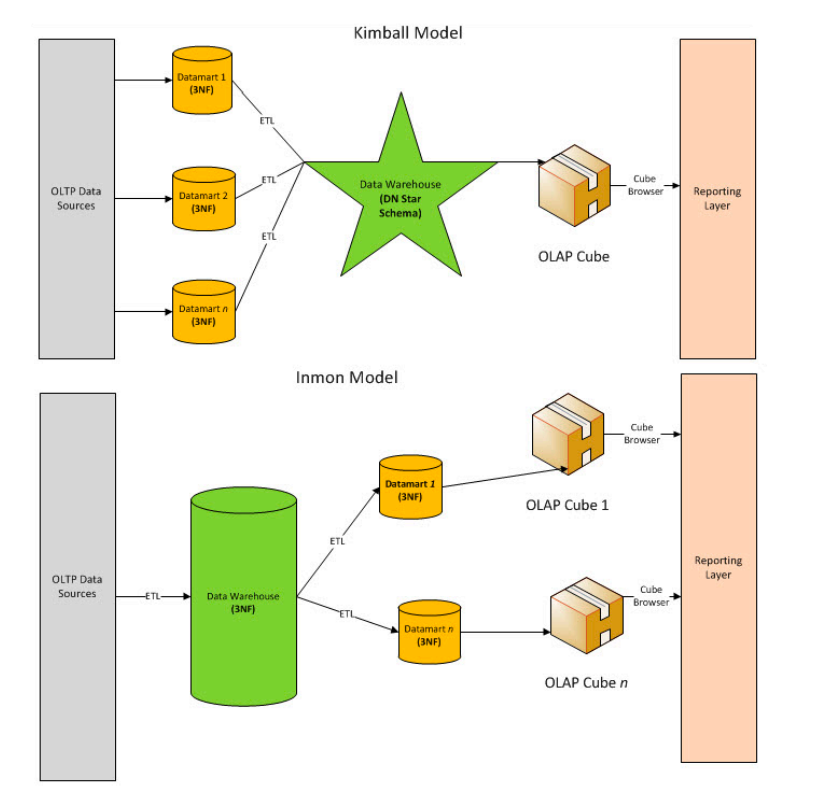
\includegraphics[width=18cm, keepaspectratio]{assets/db-places.png}
	\caption{Структуры хранилищ данных Киммбалла/Инмона} 
\end{figure}

Схемы «звезда» и «снежинка» — это два способа структурировать хранилище данных.

Схема типа «звезда» имеет централизованное хранилище данных, которое хранится в таблице фактов. Схема разбивает таблицу фактов на ряд денормализованных таблиц измерений. Таблица фактов содержит агрегированные данные, которые будут использоваться для составления отчетов, а таблица измерений описывает хранимые данные. Денормализованные проекты менее сложны, потому что данные сгруппированы. Таблица фактов использует только одну ссылку для присоединения к каждой таблице измерений. Более простая конструкция звездообразной схемы значительно упрощает написание сложных запросов.

Схема типа «снежинка» отличается тем, что использует нормализованные данные. Нормализация означает эффективную организацию данных так, чтобы все зависимости данных были определены, и каждая таблица содержала минимум избыточности. Таким образом, отдельные таблицы измерений разветвляются на отдельные таблицы измерений.

\textbf{ETL \&  ELT}

ETL и ELT — два разных способа загрузки данных в хранилище.

\textit{ETL (Extract, Transform, Load)} начала извлекают данные из пула источников данных. Данные хранятся во временной промежуточной базе данных. Затем выполняются операции преобразования, чтобы структурировать и преобразовать данные в подходящую форму для целевой системы хранилища данных. Затем структурированные данные загружаются в хранилище и готовы к анализу.

Инструменты ETL используются для интеграции данных, чтобы удовлетворить требованиям систем управления реляционными базами данных и/или традиционных хранилищ данных с поддержкой OLAP (online analytical processing, аналитической онлайн-обработки). Инструменты OLAP и запросы (SQL) требуют, чтобы массивы данных структурировались и стандартизировались при помощи серии преобразований, выполняемых до того, как данные попадут в хранилище.

\textit{ELT (Extract, Load, Transform)} анные сразу же загружаются после извлечения из исходных пулов данных. Промежуточная база данных отсутствует, что означает, что данные немедленно загружаются в единый централизованный репозиторий. Данные преобразуются в системе хранилища данных для использования с инструментами бизнес-аналитики и аналитики.

\textbf{Этапы ETL \&  ELT:}
\begin{enumerate}
	\item Процесс загрузки данных из пулла источников.
	\item Процесс валидации (отвечает за выявление ошибок и пробелов в данных).
	\item Процесс мэппинга данных.
	\item Процесс агрегации данных. Этот процесс нужен из-за разности детализации данных в OLTP и OLAP системах.
	OLTP система может содержать несколько сумм для одного и того же набора элементов справочников, a OLAP-системы — это, по сути, полностью денормализованная таблица фактов и окружающие ее таблицы справочников.
	\item Процесс выгрузки данных в целевую систему.
\end{enumerate}

\newpage

\subsection{Транзакции. Определение, свойства и уровни изоляции транзакций. Неблагоприятные эффекты, вызванные параллельным выполнением транзакци , и способы их устранения. Управление транзакциями и способы обработки ошибок}

\textbf{Транзакция} --- последовательность операций, выполняемая как единое целое. (всё или ничего).

Для поддержания целостности транзакция должна обладать четырьмя свойствами АСИД:
\begin{itemize}
	\item \textit{Атомарность}. Транзакция либо выполняется полностью либо не выполняется вовсе.
	\item \textit{Согласованность (Непротиворечивость)}. . При завершении транзакции не должны быть нарушены ограничения накладываемые на данные (например constraints в БД). Согласованность подразумевает, что система будет переведена из одного корректного состояния в другое корректное
	\item \textit{Изоляция}. Параллельно выполняемые транзакции не должны влиять друг на друга,
	например менять данные которые использует другая транзакция. Результат выполнения параллельных транзакций должен быть таким, как если бы транзакции выполнялись последовательно.
	\item \textit{Долговечность (Устойчивость)}. После фиксации изменения не должны быть утеряны.
\end{itemize}

\textbf{Транзакции классифицируются по признаку определения границ}:
\begin{enumerate}
	\item \textit{Автоматические транзакции}. В этом режиме каждая инструкция T-SQL выполняется как отдельная транзакция. Если выполнение инструкции завершается успешно, происходит фиксация; в противном случае происходит откат.
	\item \textit{Неявные транзакции}. Если соединение работает в режиме неявных транзакции, то после фиксации или отката текущей транзакции автоматически начинает новую транзакцию. В этом режиме явно указывается только граница окончания транзакции с помощью инструкций COMMIT TRANSACTION и ROLLBACK TRANSACTION
	\item \textit{Явные транзакции}.
	
	Для определения явных транзакций используются следующие инструкции:
	\begin{itemize}
		\item BEGIN TRANSACTION – задает начальную точку явной транзакции для соединения;
		\item COMMIT TRANSACTION или COMMIT WORK – используется для успешного завершения транзакции, если не возникла ошибка;
		\item ROLLBACK TRANSACTION или ROLLBACK WORK – используется для отмены транзакции, во время которой возникла ошибка.
		\item SAVE TRANSACTION – используется для установки точки сохранения или маркера внутри транзакции. Точка cохранения определяет место, к которому может возвратиться транзакция, если часть транзакции условно отменена. Если транзакция откатывается к точке сохранения, то ее выполнение должно быть продолжено до завершения с обработкой дополнительных инструкций языка T-SQL, если необходимо, и инструкции COMMIT TRANSACTION, либо транзакция должна быть полностью отменена откатом к началу. Для отмены всей транзакции следует использовать инструкцию ROLLBACK TRANSACTION; в этом случае отменяются все инструкции транзакции.
	\end{itemize}
\end{enumerate}

\textbf{Управлением параллельным выполнением транзакции}

Когда множество пользователей одновременно пытаются модифицировать данные в базе данных, необходимо создать систему управления, которая защитила бы модификации, выполняемым одним пользователем, от негативного воздействия модификаций, сделанных другими.
Выделяют два типа управления параллельным выполнением:
\begin{itemize}
	\item \textit{Пессимистическое управление параллельным выполнением}. При пессимистическом подходе первый пользователь захвативший данные препятствует получению данных остальным. Если конфликты редки разумно выбрать оптимистическую стратегию, так как она обеспечивает более высокий уровень параллелизма.
	\item \textit{Оптимистическое управление параллельным выполнением}. При оптимистическом подходе несколько пользователей получают в свое распоряжение копии данных. Первый завершивший редактирование сохраняет изменения, остальные же должны осуществить слияние изменений. Оптимистический алгоритм позволяет конфликту произойти, но система должна восстановиться после конфликта.
\end{itemize}
В случае пессимистичного управления в СУБД не реализованы механизмы блокировки, то при одновременном чтении и изменении одних и тех же данных несколькими пользователями могут возникнуть следующие проблемы одновременного доступа:
\begin{itemize}[label=---]
	\item \textbf{Проблема последнего изменения.}
	
	\begin{table}[ht!]
		\begin{center}
			\label{tbl:pr1}
			\begin{tabular}{|c|c|}
				\hline
				Транзакция 1 & Транзакция 2 \\
				\hline
				UPDATE tbl1 SET f2=f2+20 WHERE f1=1; & UPDATE tbl1 SET f2=f2+25 WHERE f1=1; \\
				\hline
			\end{tabular}
		\end{center}
	\end{table}
	В обеих транзакциях изменяется значение поля f2, по их завершении значение поля должно быть
	увеличено на 45. В действительности может возникнуть следующая последовательность действий: Обе транзакции одновременно читают текущее состояние поля. Точная физическая одновременность здесь не обязательна, достаточно, чтобы вторая по порядку операция чтения выполнилась до того, как другая транзакция запишет свой результат. Обе транзакции вычисляют новое значение поля, прибавляя, соответственно, 20 и 25 к ранее прочитанному значению. Транзакции пытаются записать результат вычислений обратно в поле f2. Поскольку физически одновременно две записи выполнить невозможно, в реальности одна из операций записи будет выполнена раньше, другая позже. При этом вторая операция записи перезапишет результат первой. 
	
	В результате значение поля f2 по завершении обеих транзакций может увеличиться не на 45, а на 20
	или 25, то есть одна из изменяющих данные транзакций «пропадёт».
	
	\item \textbf{Проблема  <<грязного>> чтения.}
	\begin{table}[ht!]
		\begin{center}
			\label{tbl:pr1}
			\begin{tabular}{|c|c|}
				\hline
				Транзакция 1 & Транзакция 2 \\
				\hline
				UPDATE tbl1 SET f2=f2+1 WHERE f1=1; & \\
				& SELECT f2 FROM tbl1 WHERE f1=1; \\
				ROLLBACK WORK; & \\
				\hline
			\end{tabular}
		\end{center}
	\end{table}
	В транзакции 1 изменяется значение поля f2, а затем в транзакции 2 выбирается значение этого
	поля. После этого происходит откат транзакции 1. В результате значение, полученное второй транзакцией, будет отличаться от значения, хранимого в базе данных.
	\item \textbf{Проблема неповторимого чтения.} Ситуация, когда при повторном чтении в рамках одной транзакции ранее прочитанные данные оказываются изменёнными.
	
	\begin{table}[ht!]
		\begin{center}
			\label{tbl:pr1}
			\begin{tabular}{|c|c|}
				\hline
				Транзакция 1 & Транзакция 2 \\
				\hline
				& SELECT f2 FROM tbl1 WHERE f1=1; \\
				UPDATE tbl1 SET f2=f2+3 WHERE f1=1; & \\
				COMMIT; & \\
				& SELECT f2 FROM tbl1 WHERE f1=1; \\
				\hline
			\end{tabular}
		\end{center}
	\end{table}
	В транзакции 2 выбирается значение поля f2, затем в транзакции 1 изменяется значение поля f2.
	При повторной попытке выбора значения из поля f2 в транзакции 2 будет получен другой результат.
	Эта ситуация особенно неприемлема, когда данные считываются с целью их частичного изменения и
	обратной записи в базу данных.
	
	\item \textbf{Проблема чтения фантомов.}
	\begin{table}[ht!]
		\begin{center}
			\label{tbl:pr1}
			\begin{tabular}{|c|c|}
				\hline
				Транзакция 1 & Транзакция 2 \\
				\hline
				& SELECT f2 FROM tbl1 WHERE f1=1; \\
				INSERT INTO tbl1 (f1,f2) VALUES (15,20); & \\
				COMMIT; & \\
				& SELECT f2 FROM tbl1 WHERE f1=1; \\
				\hline
			\end{tabular}
		\end{center}
	\end{table}
	В транзакции 2 выполняется SQL-оператор, использующий все значения поля f2. Затем в транзакции
	1 выполняется вставка новой строки, приводящая к тому, что повторное выполнение SQL-оператора
	в транзакции 2 выдаст другой результат. Такая ситуация называется чтением фантома (фантомным
	чтением). От не повторяющегося чтения оно отличается тем, что результат повторного обращения к
	данным изменился не из-за изменения/удаления самих этих данных, а из-за появления новых (фантомных) данных.
\end{itemize}

\textbf{Для решение проблем используются следующие уровни изоляции}:
\begin{itemize}
	\item \textit{Уровень 0} (read uncommitted) --- запрещение <<загрязнение>> данных (повреждение данных). Этот уровень требует, чтобы изменять данные могла только одна транзакция, а другие транзакции ожидали завершение данной транзакции.
	\item \textit{Уровень 1} (read committed) --- запрещение <<грязного>> чтения. Если транзакция начала изменение данных, то никакая другая транзакция не сможет прочитать их до завершение первой.
	\item \textit{Уровень 2} (repeatable read) --- запрещение неповторяемого чтения. Если транзакция считывает данные, то никакая другая транзакция не сможет их изменить. Таким образом, при повторном чтении они будут находится в первоначальном состоянии.
	\item \textit{Уровень 3} (snapshot, serializable)--- запрещение фантомов. Если транзакция обращается к данным, то никакая другая транзакция не сможет добавить новые или удалить имеющие строки, которые могут быть считаны при выполнении транзакции. Реализация этого уровня блокировки выполняется путем использования блокировок диапазона ключей. Подобная блокировка накладывается не на конкретные строки таблицы, а на строки удовлетворяющие определенному логическому условию.
\end{itemize}
\begin{table}[ht!]
	\begin{center}
		\label{tbl:lvl_izo}
		\begin{tabular}{|c|c|c|c|}
			\hline
			Уровень изоляции & Грязное чтение & Неповторяющееся чтение & Фантом \\
			\hline
			read uncommitted & Да & Да & Да\\
			\hline
			read committed & Нет & Да & Да\\
			\hline
			repeatable read & Нет & Нет & Да\\
			\hline
			snapshot & Нет & Нет & Нет\\
			\hline
			serializable & Нет & Нет & Нет\\
			\hline
		\end{tabular}
	\end{center}
\end{table}
При это одновременно может быть установлен только один параметр уровня изоляции, который продолжает действовать для текущего соединения до тех пор, пока не будет явно изменен.
Уровни изоляции транзакции определяют тип блокировки, применяемый к операциям считывания.
В любой момент транзакции можно переключиться с одного уровня изоляции на другой.
Тогда для транзакции изменяется уровень изоляции, ресурсы, которые считываются после изменения, защищаются в соответствии с правилами нового уровня. Ресурсы, которые считываются до изменения, остаются защищенными в соответствии с правилами предыдущего уровня.

\textbf{Способы обработки ошибок.}
Если ошибка делает невозможным успешное выполнение транзакции, SQL Server автоматически выполняет ее откат и 
освобождает ресурсы, удерживаемые транзакцией. Если сетевое соединение клиента с SQL Server разорвано, то после  того, как SQL Server получит уведомление от сети о разрыве соединения, выполняется откат всех необработанных транзакций для этого соединения. В случае сбоя клиентского приложения, выключения либо перезапуска клиентского компьютера соединение также будет разорвано, а SQL Server выполнит откат всех необработанных транзакций после получения уведомления о разрыве от сети. Если клиент выйдет из приложения, выполняется откат всех необработанных транзакций.

На случай возникновения ошибок код приложения должен содержать исправляющее действие: COMMIT или 
ROLLBACK. Эффективным средством для обработки ошибок, включая ошибки транзакций, является конструкция языка 
Transact-SQL TRY...CATCH

\newpage

\subsection{Блокировки. Определение, свойства, иерархии, гранулярность и взаимоблокировки, алгоритмы обнаружения взаимоблокировок}

\textbf{Определение}

Блокировка --- это механизм, с помощью которого компонент Database Engine
синхронизирует одновременный доступ нескольких пользователей к одному фрагменту данных.

\textbf{Свойства}

\begin{enumerate}
	\item гранулярностью (или размером блокировки)
	\item режимом (или типом блокировки)
	\item продолжительностью
\end{enumerate}

\subsubsection{Иерархии}

Компонент Database Engine часто получает блокировки на нескольких уровнях гранулярности одновременно, чтобы полностью защитить ресурс. Такая группа блокировок на нескольких уровнях гранулярности называется иерархией блокировки. Например, чтобы полностью защитить операцию чтения индекса, экземпляру компоненту Database Engine может потребоваться получить разделяемые блокировки на строки и намеренные разделяемые блокировки на страницы и таблицу.

\subsubsection{Гранулярность}

Гранулярность блокировки определяет, какой ресурс блокируется в одной попытке блокировки.

\begin{table}[ht!]
	\begin{center}
		\caption{}
		\label{tbl:gran}
		\begin{tabular}{|c|l|}
			\hline
			\textbf{Ресурс} & \textbf{Описание} \\
			\hline
			RID & Идентификатор строки, используемый для блокировки 1 строки в куче \\
			\hline
			KEY & Блокировка строки в индексе, используемая \\ & для защиты диапазонов значений ключа в
			сериализуемых транзакциях. \\
			\hline
			PAGE & 8КБ страница в базе данных, например страница данных или индекса. \\
			\hline
			EXTENT & Упорядоченная группа из восьми страниц, \\ & например страниц данных или индекса. \\
			\hline
			HOBT & Куча или сбалансированное дерево. Блокировка, защищающая индекс \\ & или кучу стр.
			данных в таблице, не имеющей кластеризованного индекса. \\
			\hline
			TABLE & Таблица полностью, включая все данные и индексы. \\
			\hline
			FILE & Файл базы данных. \\
			\hline
			APPLICATION & Определяемый приложением ресурс. \\
			\hline
			METADATA & Блокировки метаданных. \\
			\hline
			ALLOCATION\_UNIT & Единица размещения. \\
			\hline
			DATABASE & База данных, полностью. \\
			\hline
		\end{tabular}
	\end{center}
\end{table}
\FloatBarrier

\subsubsection{Взаимоблокировки}

Взаимоблокировки или тупиковые ситуации (deadlocks) возникают тогда, когда одна из транзакций не может завершить свои действия, поскольку вторая транзакция заблокировала нужные ей ресурсы, а вторая в то же время ожидает освобождения ресурсов первой транзакцией. Как SQL Server обнаруживает взаимоблокировки? Обнаружение взаимоблокировки выполняется потоком диспетчера блокировок, который периодически производит поиск по всем задачам в экземпляре компонента Database Engine.


Следующие пункты описывают процесс поиска:

\begin{enumerate}
	\item Значение интервала поиска по умолчанию составляет 5 секунд.
	\item Если диспетчер блокировок находит взаимоблокировки, интервал обнаружения взаимоблокировок снижается с 5 секунд до 100 миллисекунд в зависимости от частоты взаимоблокировок.
	
	\item Если поток диспетчера блокировки прекращает поиск взаимоблокировок, компонент Database Engine увеличивает интервал до 5 секунд.
	\item Если взаимоблокировка была только что найдена, предполагается, что следующие потоки, которые должны ожидать блокировки, входят в цикл взаимоблокировки. Первая пара элементов, ожидающих блокировки, после того как взаимоблокировка была обнаружена, запускает поиск
	взаимоблокировок вместо того, чтобы ожидать следующий интервал обнаружения взаимоблокировки. Например, если текущее значение интервала равно 5 секунд и была обнаружена взаимоблокировка, следующий ожидающий блокировки элемент немедленно приводит в действие детектор взаимоблокировок. Если этот ожидающий блокировки элемент является частью взаимоблокировки, она будет обнаружена немедленно, а не во время следующего поиска взаимоблокировок.
	\item Компонент Database Engine обычно выполняет только периодическое обнаружение взаимоблокировок. Так как число взаимоблокировок, произошедших в системе, обычно мало, периодическое обнаружение взаимоблокировок помогает сократить издержки от взаимоблокировок в системе.
	\item Если монитор блокировок запускает поиск взаимоблокировок для определенного потока, он идентифицирует ресурс, ожидаемый потоком. После этого монитор блокировок находит владельцев определенного ресурса и рекурсивно продолжает поиск взаимоблокировок для этих потоков до тех пор, пока не найдет цикл. Цикл, определенный таким способом, формирует взаимоблокировку. 
	\item После обнаружения взаимоблокировки компонент Database Engine завершает взаимоблокировку, выбрав один из потоков в качестве жертвы взаимоблокировки. Компонент Database Engine прерывает выполняемый в данный момент пакет потока, производит откат транзакции жертвы
	взаимоблокировки и возвращает приложению ошибку 1205. Откат транзакции жертвы взаимоблокировки снимает все блокировки, удерживаемые транзакцией. Это позволяет транзакциям потоков разблокироваться, и продолжить выполнение. Ошибка 1205 жертвы взаимоблокировки
	записывает в журнал ошибок сведения обо всех потоках и ресурсах, затронутых взаимоблокировкой.
\end{enumerate}

\newpage

\subsection{Журнализация. Операции журнала транзакций и его логическая и физическая архитектуры. Модели восстановления. Метаданные}

\subsubsection{Типы используемых файлов}

\begin{enumerate}
	\item Первичные файлы данных.
	\item Вторичные файлы данных.
	\item Файлы журналов.
\end{enumerate}

\subsubsection{Операции}

\begin{enumerate}
	\item Восстановление отдельных транзакций.
	\item Восстановление всех незавершенных транзакци при запуске SQL Server.
	\item Накат восстановленно базы данных, файла, файлово группы или страницы до момента сбоев.
	\item Поддержка репликации транзакций.
	\item Поддержка решений с резервными серверами.
\end{enumerate}

\subsubsection{Логическая архитектура}

На логическом уровне журнал транзакций состоит из последовательности записей. Двумя основными типами записи Log-файла являются:

\begin{enumerate}
	\item код выполненной логической операции.
	\begin{itemize}
		\item Для наката логической операции выполняется эта операция.
		\item Для отката логической операции выполняется логическая операция, обратная зарегистрированной.
	\end{itemize}
	\item исходны и результирующий образ измененных данных.
	\begin{itemize}
		\item Для наката операции применяется результирующий образ.
		\item Для отката операции применяется исходный образ.
	\end{itemize}
\end{enumerate}

\subsubsection{Физическая архитектура}

На физическом уровне журнал транзакций состоит из одного или
нескольких физических файлов. Каждый физический файл журнала
разбивается на несколько виртуальных файлов журнала (VLF). VLF не
имеет фиксированного размера. Не существует также и определенного
числа VLF, приходящихся на один физический файл журнала. Компонент
Database Engine динамически определяет размер VLF при создании или
расширении файлов журнала. Компонент Database Engine стремится
обслуживать небольшое число VLF. Администраторы не могут настраивать
или устанавливать размеры и число VLF.

Журнал транзакций является оборачиваемым файлом. Рассмотрим
пример. Пусть база данных имеет один физический файл журнала,
разделенный на четыре виртуальных файла журнала. При создании базы
данных логический файл журнала начинается в начале физического файла
журнала. Новые записи журнала добавляются в конце логического журнала
и приближаются к концу физического файла журнала. Усечение журнала
освобождает любые виртуальные журналы, все записи которых находятся
перед минимальным регистрационным номером восстановления в журнале
транзакций (MinLSN). MinLSN является регистрационным номером самой
старой записи, которая необходима для успешного отката на уровне всей базы данных. Журнал транзакций рассматриваемой в данном примере
базы данных будет выглядеть примерно так же, как на следующей
иллюстрации.

\begin{figure}[ht!]
	\centering
	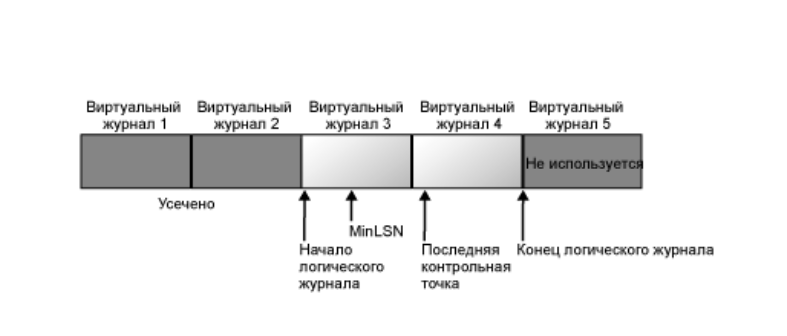
\includegraphics[width=18cm, keepaspectratio]{assets/physics.png}
	\caption{B-Tree} 
\end{figure}
\FloatBarrier

Часть журнала, начинающаяся с номера MinLSN и заканчивающаяся
последней записью,
называется активной частью журнала, или активным журналом. Этот
раздел журнала
необходим для выполнения полного восстановления базы данных. Ни одна
часть
активного журнала не может быть усечена. Все записи журнала до номера
MinLSN
должны быть удалены из частей журнала.

\subsubsection{Модель восстановления}

Модель восстановления --- это свойство базы данных, которое управляет процессом регистрации транзакций, определяет, требуется ли для журнала транзакций резервное копирование, а также определяет, какие типы операций восстановления доступны.

\begin{enumerate}
	\item Модель полного восстановления (FULL).
	\item Модель восстановления с неполным протоколированием (BULK\_LOGGED).
	\item Простая модель восстановления (SIMPLE).
\end{enumerate}

\textbf{Восстановление данных}

\begin{enumerate}
	\item База данных (полное восстановление базы данных).
	\item Файл данных (восстановление файла).
	\item Страница данных (восстановление страницы).
\end{enumerate}

\textbf{Метаданные}

Метаданные, в общем случае, это данные о данных, информация об информации, описание контента.

Метаданные, в общем случае, это данные о данных, информация об
информации, описание контента. Каждая СУБД сохраняет метаданные обо
всех сущностях базы данных. Так в SQL Server с помощью инструкции
CREATE можно создать 52 сущности.

В разных СУБД применяются разные названия для метаданных -
системный каталог, словарь данных и др. Однако общим свойством всех
современных реляционных СУБД является то, что каталог/словарь сам
состоит из таблиц, а точнее - системных таблиц. В результате пользователь
может обращаться к метаданным так же, как и к прикладным данным,
используя инструкцию SELECT. Изменения же в каталоге/словаре
производятся автоматически при выполнении пользователем инструкций,
изменяющих состояние объектов базы данных. Системные таблицы не
должны изменяться непосредственно ни одним пользователем. Например,
не стоит изменять системные таблицы с помощью инструкций DELETE,
UPDATE или INSERT либо с помощью пользовательских триггеров.
Обращение к документированным столбцам системных таблиц разрешено.
Однако многие столбцы системных таблиц не документированы. В
приложениях непосредственные запросы к недокументированным
столбцам применять не следует. Чтобы исключить прямой доступ к
системным таблицам, пользователь «видит» не сами таблицы, а созданные
на их базе представления, которые он, конечно же, не может изменять.
Состав и структура каталога/словаря очень различны для различных СУБД.

\textbf{Microsoft SQL Server} предоставляет следующие коллекции системных
представлений, содержащие метаданные:

\begin{enumerate}
	\item Представления информационной схемы
	\item Представления каталога
	\item Представления совместимости
	\item Представления репликации
	\item Динамические административные представления и функции
	\item Представления приложения уровня данных (DAC)
\end{enumerate}

\newpage

\subsection{Безопасность и Аудит. Ключевые понятия и участники системы безопасности. Модели управления доступом}

SQL Server обеспечивает защиту данных от неавторизированного
доступа и от фальсификации. \textbf{Основными} функциями безопасности
SQL Server являются:

\begin{enumerate}
	\item проверка подлинности (аутентификация) – процедура проверки
	соответствия некоего лица и его учетной записи в компьютерной
	системе. Один из способов аутентификации состоит в задании
	пользовательского идентификатора, в просторечии называемого
	«логином» (login – регистрационное имя пользователя) и пароля –
	некой конфиденциальной информации, знание которой обеспечивает
	владение определенным ресурсом. Аутентификацию не следует путать с идентификацией. Идентификация – это установление личности самого физического лица (а не его виртуальной учетной записи, коих может быть много).
	\item авторизация --- это предоставление лицу прав на какие-то действия в
	системе.
\end{enumerate}


\textbf{Дополнительными} функциями безопасности SQL Server являются:

\begin{enumerate}
	\item шифрование,
	\item контекстное переключение,
	\item олицетворение,
	\item встроенные средства управления ключами.
\end{enumerate}

В основе \textbf{системы безопасности} SQL Server лежат три понятия:

\begin{enumerate}
	\item участники системы безопасности (Principals);
	\item защищаемые объекты (Securables),
	\item система разрешений (Permissions).
\end{enumerate}

\subsubsection{Участники системы безопасности}

Участники системы безопасности или принципалы – это сущности, которые
могут запрашивать ресурсы SQL Server.

Принципалы могут быть иерархически упорядочены. Область влияния
принципала зависит

\begin{enumerate}
	\item от области его определения: Windows, SQL Server, база данных,
	\item от того, коллективный это участник или индивидуальный. Имя входа
	Windows является примером индивидуального (неделимого) участника,
	а группа Windows — коллективного. При создании учетной записи SQL
	Server ей назначается идентификатор и идентификатор безопасности. В
	представлении каталога sys.server\_principals они отображаются в
	столбцах principal\_id и SID. Участники уровня Windows – это a) Имя
	входа домена Windows, b) Локальное имя входа Windows. Участники
	уровня SQL Server – это a) Имя входа SQL Server, b) Роль сервера.
	Участники уровня базы данных – это a) Пользователь базы данных, b)
	Роль базы данных, c) Роль приложения.
\end{enumerate}

\textbf{Замечания}

\begin{enumerate}
	\item Имя входа «sa» SQL Server. Имя входа sa SQL Server является
	участником уровня сервера. Оно создается по умолчанию при установке
	экземпляра. В SQL Server для имени входа sa базой данных по умолчанию
	будет master.
	\item Роль базы данных public. Каждый пользователь базы данных является
	членом роли базы данных public. Если пользователю не были
	предоставлены или запрещены особые разрешения на защищаемый
	объект, то он наследует на него разрешения роли public.
	\item Пользователи INFORMATION\_SCHEMA и sys. Каждая база данных
	включает в себя две сущности, которые отображены в представлениях
	каталога в виде пользователей: INFORMATION\_SCHEMA и sys. Они
	необходимы для работы SQL Server; эти пользователи не являются
	участниками и не могут быть изменены или удалены.
\end{enumerate}

\subsubsection{Защищаемые объекты}

Защищаемые объекты – это ресурсы, доступ к которым регулируется
системой авторизации. Некоторые защищаемые объекты могут храниться
внутри других, создавая иерархии «областей», которые сами могут
защищаться. К областям защищаемых объектов относятся (a) сервер, (b)
база данных и (c) схема. Далее введем следующие ограничения:

\begin{enumerate}
	\item для области «сервер» ограничимся рассмотрением вопросами
	управления учетными записями подключения (login),
	\item для области «база данных» ограничимся рассмотрением вопросами
	управления
	
	\begin{itemize}
		\item учетными записями пользователей (user),
		\item ролями (role),
		\item ролями приложений (application role).
	\end{itemize}
	
	\item для области «схема» ограничимся рассмотрением вопросами
	управления разрешениями на
	
	\begin{itemize}
		\item функции (function),
		\item процедуры (stored procedure),
		\item таблицы (table),
		\item представления (view).
	\end{itemize}

\end{enumerate}

\subsubsection{Разрешения}

У субъекта системы есть только один путь получения доступа к объектам -
иметь назначенные непосредственно или опосредовано разрешения. При
непосредственном управлении разрешениями они назначаются субъекту
явно, а при опосредованном разрешения назначаются через членство в
группах, ролях или наследуются от объектов, лежащих выше по цепочке
иерархии. Управление разрешениями производится путем выполнения
инструкций языка DCL (Data Control Language): GRANT (разрешить), DENY
(запретить) и REVOKE (отменить).

\subsubsection{Аудит SQL Server}

Начиная с версии SQL Server 2008 в редакции Enterprise вводится аудит
SQL Server Audit – функциональность системы безопасности, которая
может отслеживать практически любое действие с сервером или базой
данных (выполняемое пользователями) и записывать эти действия в
файловую систему или системный журнал Windows.

\subsubsection{Система управления на основе политик}

Одна из новых возможностей, появившаяся в SQL Server 2008, – система
управления на основе политик (Policy-Based Management), которая
позволяет создавать политики для обеспечения соответствия нормативам
управления базой данных.

Система управления на основе политик позволяет администратору баз
данных (АБД) создавать политики для управления объектами и
экземплярами базы данных. Эти политики дают АБД возможность
устанавливать правила создания и изменения объектов и их свойств. С
помощью новой системы можно, например, создать политику уровня БД,
запрещающую использование для БД свойства AutoShrink. Другой пример –
политика, в соответствии с которой все имена табличных триггеров в
таблице БД начинаются с tr\_.

Система управления на основе политик предусматривает использование
новых терминов и понятий. Основными из них являются:

\begin{enumerate}
	\item Политика (Policy) – набор условий, определенных аспектами цели
	управления. Другими словами, политика — это набор правил для свойств
	БД или серверных объектов.
	\item Цель управления (Target) – объект, управляемый данной системой. Сюда относятся такие объекты, как экземпляр БД, база данных, таблица, хранимая процедура, триггер, индекс.
	\item Аспект (Facet) – свойство объекта (цели управления), которое
	используется системой управления на основе политик. Например, имя
	триггера или свойство базы данных AutoShrink.
	\item Условие (Condition) – критерий для аспектов цели управления. Например,
	можно создать для факта условие, по которому все имена хранимых
	процедур в схеме «Banking» должны начинаться с bnk\_.
	Кроме того, политику можно связать с определенной категорией, что
	позволяет осуществлять управление набором политик, привязанных к той
	же самой категории. Политика может принадлежать только к одной
	категории.
\end{enumerate}

\subsubsection{Режим оценки политик}

Существует несколько режимов оценки политик:

\begin{enumerate}
	\item По запросу (On demand) – оценку политики запускает непосредственно
	администратор.
	\item При изменении: запретить (On change: prevent) – для предотвращения
	нарушения политики используются триггеры DDL.
	\item При изменении: только внесение в журнал (On change: log only) – для проверки политики при изменении используются уведомления о событии.
	\item По расписанию (On schedule) – для проверки политики на нарушения
	используется задание агента SQL (SQL Agent).
\end{enumerate}

\subsubsection{Преимущества системы управления на основе политик}

Система управления на основе политик позволяет АБД в полной мере контролировать процессы, происходящие в базе данных. Администратор
получает возможность реализовать принятые в компании политики на уровне БД. Политики, принятые только на бумаге, помогают определить основные принципы управления базой данных и могут служить прекрасным руководством к действию, но воплощать их в жизнь очень нелегко. Для обеспечения строгого соответствия БД принятым нормативом АБД приходится пристально следить за ее повседневным использованием и функционированием. Система управления на основе политик позволяет раз и навсегда выработать политики управления и быть уверенным в том, что они будут применяться постоянно и в полном объеме.

\newpage

\subsection{MPP системы. Распределенное и колоночное хранение. Распределенные вычисления, модель MapReduce. Обеспечение отказоустойчивости.}

\subsubsection{Массивно-параллельные системы обработки (massively parallel processing, MPP).}

Хотя архитектуры отдельных поставщиков могут варьироваться, массивно-
параллельная обработка — наиболее развитой, проверенный и широко используемый механизм хранения и анализа больших объемов данных. Так что же собой
представляет массивно-параллельная архитектура и что в ней особенного?
При использовании массивно-параллельной архитектуры данные
разделяются на фрагменты, обрабатываемые независимыми
центральными процессорами (CPU) и хранящиеся на разных носителях.
Это похоже на загрузку разных фрагментов данных на несколько
объединенных в сеть персональных компьютеров. Таким образом
устраняется ограничение, обусловленное наличием одного центрального
сервера с одним процессором и диском. Данные в массивнопараллельной
системе распределяются по нескольким дискам, управляемым
процессорами разных серверов.

\begin{figure}[ht!]
	\centering
	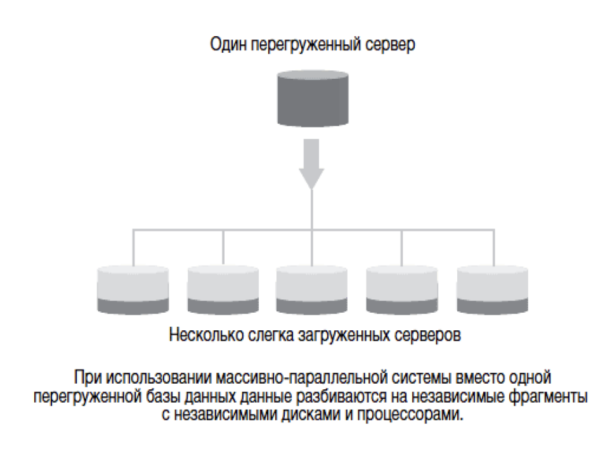
\includegraphics[width=18cm, keepaspectratio]{assets/MPP-1.png}
	\caption{} 
\end{figure}
\FloatBarrier

\begin{figure}[ht!]
	\centering
	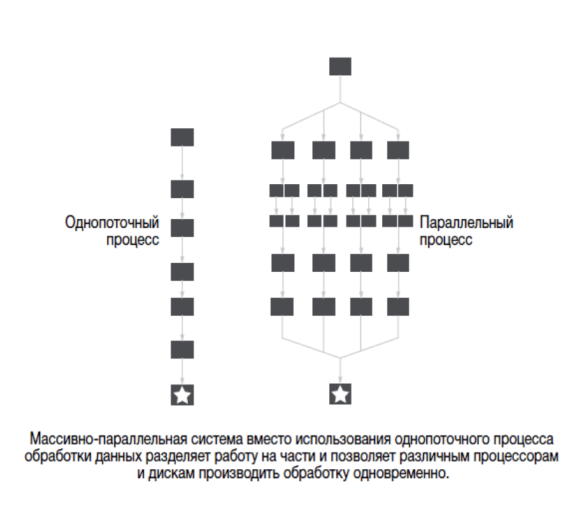
\includegraphics[width=18cm, keepaspectratio]{assets/MPP-2.png}
	\caption{} 
\end{figure}
\FloatBarrier

При использовании MPP-систем данные не хранятся в одном месте, что
облегчает
восстановление в случае выхода оборудования из строя.

\subsubsection{Аппаратная архитектура на примере VERTICA}

Рассмотрим Vertica на уровне кластера. Эта СУБД обеспечивает массивно-
параллельную
обработку данных (МРР) в распределенной вычислительной архитектуре —
«shared-nothing» — где, в принципе, любая нода готова подхватить функции
любой другой ноды. 

\textbf{Основные свойства:}

\begin{enumerate}
	\item отсутствует единая точка отказа,
		\item каждый узел независим и самостоятелен,
			\item отсутствует единая для всей системы точка подключения,
				\item узлы инфраструктуры дублируются,
		\item данные на узлах кластера автоматически копируются.
\end{enumerate}

Кластер без проблем линейно масштабируется. Мы просто ставим сервера
в полку и
подключаем их через графический интерфейс. Помимо серийных серверов,
возможно развертывание на виртуальные машины. Что можно добиться \textbf{с помощью
расширения}?

\begin{enumerate}
	\item Увеличения объема для новых данных
	\item Увеличение максимальной рабочей нагрузки
	\item Повышение отказоустойчивости. Чем больше нод в кластере, тем меньше
	вероятность
	выхода кластера из строя из-за отказа, а следовательно, тем ближе мы к
	обеспечению
	доступности 24/7.
\end{enumerate}

Периодически ноды нужно вынимать из кластера для обслуживания. Еще
довольно
распространенный кейс в крупных организация — сервера сходят с
гарантии и переходят из продуктивной в какую-нибудь тестовую среду. На
их место встают новые, которые находятся на гарантии производителя. По
итогам всех этих операций нужно выполнять ребалансировку.
Это процесс, когда данные перераспределяются между нодами —
соответственно
перераспределяется рабочая нагрузка. Это требовательный к ресурсам
процесс, и на
кластерах с большим объемом данных он может сильно снизить
производительность. Чтобы этого избежать, нужно выбрать сервисное окно
— время, когда нагрузка минимальна, и в этом случае пользователи этого
не заметят.

\subsubsection{Проекции}

Для понимания, как хранятся данные в Vertica, требуется разобраться с
одним из основных понятий — проекцией.

Логические единицы хранения информации — это схемы, таблицы и
представления.

Физические единицы — это проекции. \textbf{Проекции} бывают нескольких типов:

\begin{enumerate}
	\item суперпроекции (Superprojection),
	\item запрос-ориентированные проекции (Query-Specific Projections),
	\item агрегированные проекции (Aggregate Projections).
\end{enumerate}

При создании любой таблицы автоматически создается суперпроекция,
которая содержит все колонки нашей таблицы. Если нужно ускорить какой-
то из регулярных процессов, мы можем создать специальную запрос-
ориентированную проекцию, которая будет содержать, допустим, 3 столбца
из 10.

Для ускорения предназначен и третий тип — агрегированные проекции. Не
буду вдаваться в их подклассы — это не очень интересно. Сразу хочу
предупредить, что постоянно решать свои проблемы с выполнением
запросов через создание новых проекций не стоит. В конечном итоге
кластер начнет тормозить.

Создавая проекции, нужно оценивать, хватает ли нашим запросам
суперпроекций. Если мы все-таки хотим поэкспериментировать, добавляем
строго по одной новой проекции. При возникновении проблем так будет
проще найти первопричину. Для больших таблиц следует создавать
сегментированную проекцию. Она разбивается на сегменты, которые
распределяются по нескольким нодам, что повышает отказоустойчивость и
минимизирует
нагрузки на одну ноду. Если таблички маленькие, то лучше делать
несегментированные
проекции. Они полностью копируются на каждую ноду, и
производительность таким образом увеличивается. Оговорюсь: в терминах
Vertica «маленькая» таблица — это примерно 1 млн строк.

\begin{figure}[ht!]
	\centering
	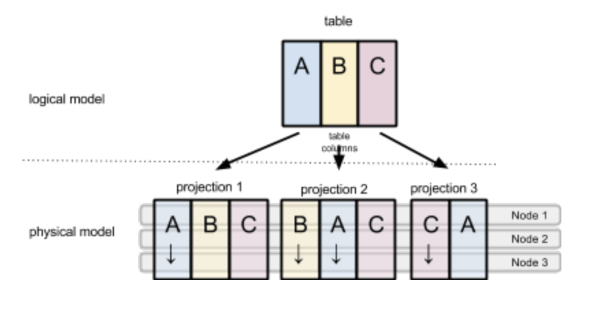
\includegraphics[width=18cm, keepaspectratio]{assets/MPP-3.png}
	\caption{} 
\end{figure}
\FloatBarrier

\subsubsection{Отказоустойчивость}

Отказоустойчивость в Vertica реализована при помощи механизма K-Safety.
Он довольно
простой с точки зрения описания, но сложный с точки зрения работы на
уровне движка. Им можно управлять с помощью параметра K-Safety — он
может иметь значение 0, 1 или 2. Этот параметр задает количество копий
сегментированных проекционных данных.

Копии проекций называются buddy projections. Я попытался перевести это
словосочетание через Яндекс-переводчик и получилось что-то вроде
«проекции-кореша». Гугл предлагал варианты и интересней. Обычно
данные проекции называют партнерскими или соседними, по их
функциональному назначению. Это проекции, которые просто хранятся на
соседних нодах и таким образом резервируются. У несегментированных
проекций нет buddy projections — они копируются полностью.

\begin{figure}[ht!]
	\centering
	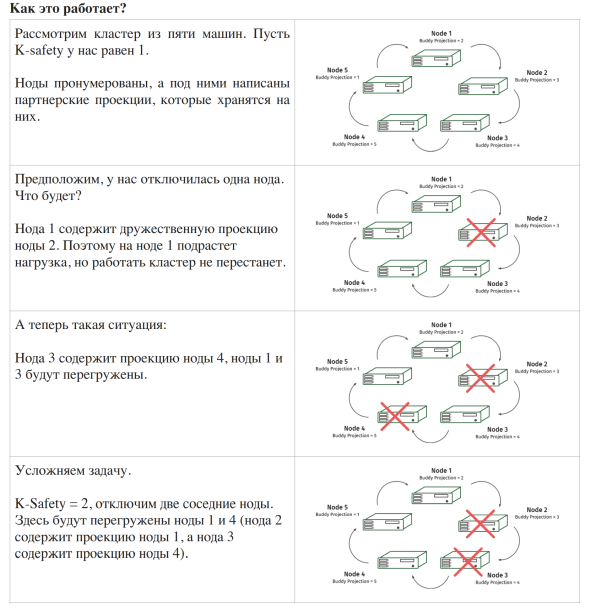
\includegraphics[width=18cm, keepaspectratio]{assets/MPP-4.png}
	\caption{} 
\end{figure}
\FloatBarrier

\subsubsection{В чем выгода колоночного хранения?}

Если мы читаем строки, то, например, для выполнения команды
SELECT 1,11,15 FROM table1
нам придется читать всю таблицу. Это огромный объем информации.

В данном случае колоночный подход выгоднее. Он позволяет считать
только три нужных нам столбца, экономя память и время.

\begin{figure}[ht!]
	\centering
	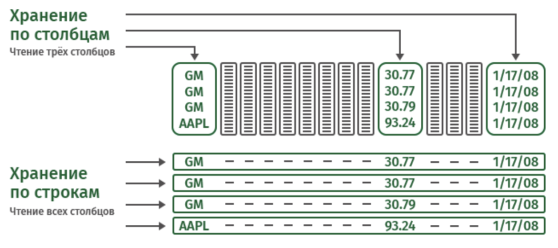
\includegraphics[width=18cm, keepaspectratio]{assets/MPP-5.png}
	\caption{} 
\end{figure}
\FloatBarrier

\textbf{MapReduce} — это способ агрегации больших хранилищ данных. Стадия
Map выполняется на множестве серверных узлов распределенной
обработки. Она обычно исполняет некую задачу на каждом
распределенном серверном узле для выборки данных из узлов данных и
может дополнительно преобразовывать или предварительно обрабатывать
данные, когда они находятся на распределенной серверном узле. Стадия
Reduce выполняется на одном или более серверных узлов конечной
обработки и консолидирует все результаты от стадий Map в один конечный
набор результатов, используя иножество различных алгоритмов
объединения.

Одно из основных преимуществ MapReduce — он обеспечивает
горизонтальное масштабирование (scale out) вместо вертикального (scale
up). Иначе говоря, для масштабирования вы просто добавляете обычные
серверные узлы, а не приобретаете более эффективное оборудование для
одного основного серверного узла. Горизонтальное масштабирование, в
целом, является более дешевым и гибким выбором, поскольку
используется недорогое стандартное аппаратное обеспечение, тогда как
вертикальное масштабирование обычно гораздо дороже, потому что
стоимость аппаратного обеспечения растет по экспоненте по мере
увеличения его сложности.

\newpage

\subsection{In-Memory базы данных. Преимущества и недостатки. Примеры использования}

Как это обычно бывает, у термина In-Memory DataBase нет устойчивого
русского
перевода, это что-то вроде «базы данных в оперативной памяти».
Базы данных in-memory хранятся в оперативной памяти сервера.
Очевидно, что это
обеспечивает большие преимущества в скорости, поскольку операции с
данными в
памяти выполняются меньшим числом инструкций процессора.

В терминах ACID базы данных in-memory конечно \textbf{жертвуют надежностью},
ведь при
обесточивании или перезагрузке в них пропадают все данные.
Существуют ряд методов, которые позволяют снизить этот риск:

\begin{enumerate}
	\item Снэпшоты
	\item Логи транзакций
	\item Использование NVRAM или NVDIMM
\end{enumerate}

\textbf{Redis} – быстрое хранилище в памяти с открытым исходным кодом для
структур данных
«ключ-значение». Redis поставляется с набором разнообразных структур
данных в
памяти, что упрощает создание различных специальных приложений.
Несколько фактов о ключах:
 
\begin{enumerate}
	\item Плохая идея - хранить слишком длинные ключи.
	\item Хорошая идея — придерживаться схемы при построении ключей:
	«object-type:id:field».
\end{enumerate}

\textbf{Преимущества In-Memory DataBase}

\begin{enumerate}
	\item Высокая производительность
	\item Структуры данных в памяти
	\item Универсальность и простота использования
	\item Репликация и сохранность
	\item Поддержка удобного языка разработки
\end{enumerate}

\textbf{Примеры использования In-Memory DataBase}

\begin{enumerate}
	\item Кэширование
	\item Управление сессиями
	\item Таблицы лидеров в режиме реального времени
	\item Ограничение интенсивности
	\item Очереди
	\item Чат и обмен сообщениями
\end{enumerate}
 
 
\newpage

\subsection{Инструкции языка описания данных, инструкции языка обработки данных, инструкции безопасности, инструкции управления транзакциями}

\textbf{Инструкции языка описания данных}

Описание данных: \textbf{Data Definition Language (DDL)}
– это группа операторов описания данных. Другими словами, с помощью операторов, входящих в эту группы, мы определяем структуру базы данных и работаем с объектами этой базы, т. е. создаем, изменяем и удаляем их.
\begin{itemize}
	\item CREATE — создает объект базы данных. 
	\item ALTER — изменяет объект базы данных.
	\item DROP — удаляет объект базы данных. 
	\item ENABLE TRIGGER — включает триггер DML, DDL или logon. 
	\item DISABLE TRIGGER — отключает триггер. 
	\item TRUNCATE TABLE — удаляет все строки в таблице, не записывая в журнал удаление отдельных строк. 
	\item UPDATE STATISTICS — обновляет статистику оптимизации запросов для таблицы или индексированного представления.
\end{itemize}

\textbf{Инструкции языка обработки данных}

Обработка данных: \textbf{Data Manipulation Language (DML)} – это группа операторов для манипуляции данными. С помощью этих операторов мы можем добавлять, изменять, удалять и выгружать данные из базы, т. е. манипулировать ими.

\begin{enumerate}
	\item SELECT — читывает данные, удовлетворяющие заданным условиям.
	\item INSERT — обавляет новые данные.
	\item UPDATE — изменяет существующие данные.
	\item DELETE — удаляет данные.
	\item MERGE — выполняет операции вставки, обновления или удаления для целевой таблицы на основе результатов соединения с исходной таблицей. Если условие, по которому происходит объединение — истина, то можно выполнить обновление или удаление, иначе — вставку.
	
	\begin{lstlisting}[label=updatetext]
		MERGE <Основная таблиц>
		USING <Таблица или запрос источника>
		ON <Условия объединения>
		[ WHEN MATCHED [ AND <Доп. условие> ]]
		THEN < UPDATE и л и DELETE >
		[ WHEN NOT MATCHED [ AND Доп. условие> ]
		THEN < INSERT > ]
		[ WHEN NOT MATCHED BY SOURCE [ AND <Доп. условие> ]
		THEN < UPDATE или DELETE > ] [ ... n ]
		[ OUTPUT ]
		;
	\end{lstlisting}
	
	
	\item BULK INSERT — полняет импорт файла данных в таблицу или представление базы данных в формате, указанном пользователем.
	\item READTEXT — итывает значения text, ntext или image из столбцов типа text, ntext или image начиная
	с указанной позиции
	\item WRITETEXT — обновляет и заменяет все поле text, ntext или image
	Базы данных
	\item UPDATETEXT — обновляет часть поля text, ntext или imag
\end{enumerate}

\begin{lstlisting}[label=updatetext]
	READTEXT { table . column text_ptr offset size } [ HOLDLOCK ]
	
	UPDATETEXT [ BULK ] { table_name . dest_column_name dest_text_ptr }
	{ NULL | insert_offset }
	{ NULL | delete_length }
	[ WITH LOG ]
	[ inserted_data
	| { table_name . src_column_name src_text_ptr } ]
	
	WRITETEXT [ BULK ]
	{ table . column text_ptr }
	[ WITH LOG ] { data }
\end{lstlisting}

\clearpage
\textbf{Инструкции безопасности}

Инструкции безопасности (ранее: доступа к данным): \textbf{Data Control Language (DСL)}.

SQL Server обеспечивает защиту данных от неавторизированного доступа и от фальсификации. Основными функциями безопасности SQL Server являются:
\begin{itemize}
	\item проверка подлинности (аутентификация) – процедура проверки соответствия некоего лица и его учетной записи в компьютерной системе. Один из способов аутентификации состоит в задании пользовательского идентификатора, в просторечии называемого «логином» (login – регистрационное имя пользователя) и пароля – некой конфиденциальной информации, знание которой обеспечивает владение определенным ресурсом.
	\item авторизация – это предоставление лицу прав на какие-то действия в системе.
	В основе системы безопасности SQL Server лежат три понятия:
\end{itemize}

В основе системы безопасности SQL Server лежат три понятия:
\begin{itemize}
	\item участники системы безопасности (Principals);
	\item защищаемые объекты (Securables);
	\item система разрешений (Permissions).
\end{itemize}

Участники системы безопасности или принципалы – это сущности, которые могут запрашивать ресурсы SQL Server.

Защищаемые объекты – это ресурсы, доступ к которым регулируется системой авторизации.

Инструкции безопасности:
\begin{itemize}
	\item GRANT — предоставляет пользователю разрешения на определенные операции с объектом.
	\item REVOKE — отзывает ранее выданные разрешения.
	\item DENY — задает запрет, имеющий приоритет над разрешением.
	\item ADD SIGNATURE — добавляет цифровую подпись для хранимой процедуры, функции, сборки или
	триггера.
	\item OPEN MASTER KEY — открывает главный ключ в текущей базе данных.
	\item CLOSE MASTER KEY — закрывает главный ключ в текущей базе данных.
	\item OPEN SYMMETRIC KEY — расшифровывает симметричный ключ и делает его доступным для использования.
	\item CLOSE SYMMETRIC KEY — закрывает симметричный ключ или все симметричные ключи, открытые
	в текущем сеансе.
	\item EXECUTE AS — контекст выполнения сеанса переключается на заданное имя входа и имя пользователя.
	\item REVERT — переключает контекст выполнения в контекст участника, вызывавшего последнюю инструкцию EXECUTE AS.
	\item SETUSER — позволяет члену предопределенной роли сервера sysadmin или члену предопределенной роли базы db\_owner олицетворять
	другого пользователя.
\end{itemize}

\textbf{Инструкции управления транзакциями}

\textbf{Transaction Control Language (TCL)} – группа операторов для управления транзакциями.

\textbf{Транзакция} – это команда или блок команд (инструкций), которые успешно завершаются как единое целое, при этом в базе данных все внесенные изменения фиксируются на постоянной основе или отменяются, т. е. все изменения, внесенные любой командой, входящей в транзакцию, будут отменены.
\begin{itemize}
	\item BEGIN DISTRIBUTED TRANSACTION — запускает распределенную транзакцию, управляемую координатором распределенных транзакций.
	\item BEGIN TRANSACTION — отмечает начальную точку явной локальной транзакции.
	\item COMMIT TRANSACTION — отмечает успешное завершение явной или неявной транзакции.
	\item COMMIT WORK — действует так же, как и инструкция COMMIT TRANSACTION.
	\item ROLLBACK TRANSACTION — откатывает явные или неявные транзакции до начала или до точки
	сохранения транзакции.
	\item ROLLBACK WORK — действует так же, как и инструкция ROLLBACK TRANSACTION.
	\item SAVE TRANSACTION — устанавливает точку сохранения внутри транзакции.
\end{itemize}

\newpage

\subsection{Объекты базы данных: функции, процедуры, триггеры и курсоры}

\newpage

\subsection{Оптимизация запроса: индексы, партиционирование, сегментирование}

\subsubsection{Индексы}
\textit{(материал на основе SQL Server)}

Индекс – это объект базы данных, обеспечивающий дополнительные способы быстрого поиска и извлечения данных. Индекс может создаваться на одном или нескольких столбцах. 
Это означает, что индексы бывают простыми и составными. Если в таблице нет индекса, то поиск нужных строк выполняется простым сканированием по всей таблице. При наличии индекса время поиска нужных строк можно существенно уменьшить. 

К недостаткам индексов следует отнести:
\begin{itemize}
	\item дополнительное место на диске и в оперативной памяти, 
	\item замедляются операции вставки, обновления и удаления записей. 
\end{itemize}

В SQL Server (и, наверное, многих других СУБД) индексы хранятся в виде сбалансированных деревьев. Представление индекса в виде сбалансированного дерева означает, что стоимость поиска любой строки остается относительно постоянной, независимо от того, где находится эта строка. 

\begin{figure}[ht!]
	\centering
 	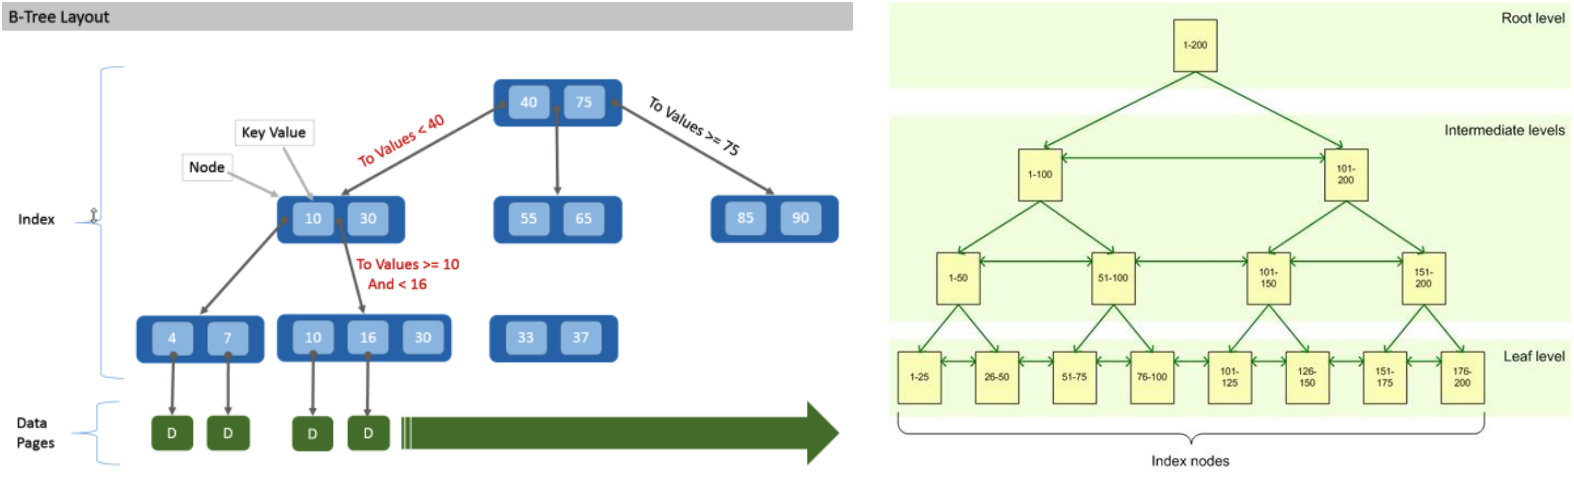
\includegraphics[width=18cm, keepaspectratio]{assets/index.png}
	\caption{B-Tree} 
\end{figure}
\FloatBarrier
Существует два типа индексов: 

\begin{itemize}
	\item Кластерные индексы
	\item Некластерные индексы, которые включают: 
	\begin{itemize}[label=--]
		\item индексы на основе кучи;
		\item индексы на основе кластерных таблиц.
	\end{itemize}
\end{itemize}

\textbf{Кластерные индексы}

В кластерном индексе таблица представляет собой часть индекса, или индекс представляет собой часть таблицы в зависимости от вашей точки зрения. Листовой узел кластерного индекса – это страница таблицы с данными. Поскольку сами данные таблицы являются частью индекса, для таблицы может быть создан только один кластерный индекс. Кластерный индекс является уникальным индексом по определению.

\textbf{Некластерные индексы на основе кучи}

В листьях некластерного индекса на основе кучи хранятся указатели на строки данных. Указатель строится на основе идентификатора файла (ID), номера страницы и номера строки на странице. Весь указатель целиком называется идентификатором строки (RID).

\textbf{Некластерные индексы, основанные на кластерных таблицах}

В листьях некластерного индекса, основанного на кластерных таблицах, хранятся указатели на корневые узлы кластерных индексов. Поиск в таком индексе состоит из двух этапов:

\begin{itemize}
	\item поиск в некластерном индексе;
	\item поиск в кластерном индексе.
\end{itemize}

\textbf{Создание индекса}

В SQL Server индексы создаются при помощи команды \textbf{CREATE INDEX}.

Помимо этого, индексы создаются при добавлении некоторых ограничений. Такой тип индексов часто называют <<связанными индексами>>. Связанные индексы создаются при добавлении одного из следующих двух типов ограничений: 
\begin{itemize}
	\item ограничения первичного ключа (PRIMARY KEY); 
	\item ограничения уникальности (UNIQUE). 
\end{itemize}

\subsubsection{Партиционирование}
\textit{(материал на основе PostgreSQL)}

Партиционирование – это метод разделения больших (исходя из количества записей, а не столбцов) таблиц на много маленьких.

Для произведения партиционирования нужно решить, каким будет ключ партиционирования – другими словами, по какому алгоритму будут выбираться партиции. Есть пара наиболее очевидных: 
\begin{enumerate}
	\item партиционирование по дате – например, выбирать партиции, основываясь на годе, в котором пользователь был создан.
	
	\textit{Достоинства:}
	\begin{itemize}[label=--]
		\item легко понять;
		\item количество строк в данной таблице будет достаточно стабильным.
	\end{itemize}
	
	\textit{Недостатки:}
	\begin{itemize}[label=--]
		\item требует поддержки – время от времени нам придётся добавлять новые партиции;
		\item поиск по имени пользователя или id потребует сканирования всех партиций;
	\end{itemize}
	
	\item партиционирование по диапазону идентификаторов – например, первый миллион пользователей, второй миллион пользователей, и так далее
	
	\textit{Достоинства:}
	\begin{itemize}[label=--]
		\item легко понять;
		\item количество строк в данной таблице будет абсолютно стабильным.
	\end{itemize}
	
	\textit{Недостатки:}
	\begin{itemize}[label=--]
		\item требует поддержки – время от времени нам придётся добавлять новые партиции;
		\item поиск по имени пользователя потребует сканирования всех партиций; 
	\end{itemize}
	
	\item партиционирование по чему-нибудь другому – например, по первой букве имени пользователя. 
	
	\textit{Достоинства:}
	\begin{itemize}[label=--]
		\item легко понять;
		\item никакой поддержки --- есть строго определенный набор партиций и нам никогда не придется добавлять новые;
	\end{itemize}
	
	\textit{Недостатки:}
	\begin{itemize}[label=--]
		\item количество строк в партициях будет стабильно расти; 
		\item в некоторых партициях будет существенно больше строк, чем в других (больше людей с никами, начинающимися на <<t*>>, чем на <<y*>>); 
		\item поиск по id потребует сканирования всех партиций;
	\end{itemize}
	
	\item есть еще пара других, не так часто используемых вариантов, вроде «партиционирования по
	хэшу от имени пользователя». 
	
\end{enumerate}

\textbf{Пример}

\begin{lstlisting}
	CREATE TABLE measurement (	
	city_id int not null,
	logdate date not null,
	peaktemp int,
	unitsales int
	) PARTITION BY RANGE (logdate);
\end{lstlisting}

\subsubsection{Сегментирование}
\textit{(материал на основе Vertica)}

Для распределения данных по кластерам используется их сегментация(Segmentation), а точнее сегментация проекций(Projection) в которых они находятся. Задача разработчика --- подобрать такой список полей и/или такую функцию(например, хэш-функцию), благодаря которым данные равномерно распределятся по нодам кластера. HP Vertica рекомендует
использовать встроенные функции HASH и MODULARHASH для этих целей. 

\textit{Прим.} Для справки: \textit{K-Safety} --- критерий отказоустойчивости БД, определяющий без какого кол-ва узлов БД сможет функционировать корректно. Он может быть равен 0, 1 или 2.

Для обеспечения K-Safety > 0 создаются сообщные проекции(Buddy Projection). Проекции называются сообщными, если они имеют в себе одинаковые наборы полей и одинаковое выражение сегментации, но хранятся на разных нодах. Сообщные проекции позволяют создать те самые реплики, которые позволяют работать БД в выбранном режиме K-Safety. 

\textbf{Пример}

\begin{figure}[h]
	\centering
	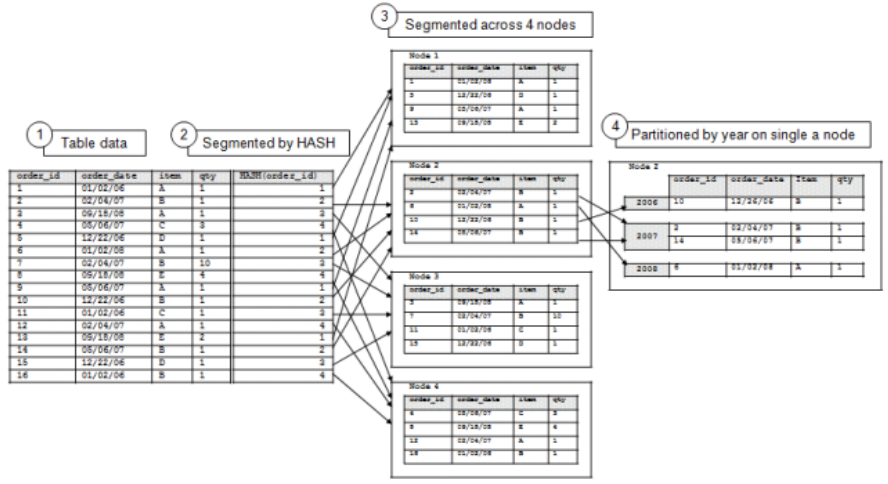
\includegraphics[width=18cm, keepaspectratio]{assets/segm.png}
	\caption{Сегментирование и партиционирование вместе} 
\end{figure}

\newpage

\subsection{План запроса. Этапы выполнения запроса}

\textbf{Ждет своего часа}.
